Each explanation in the sequence will be non-redundant and hence as small as possible. Yet, in our earlier work we noticed that some explanations were still quite hard to understand, mainly since a clue had to be combined with implicit constraints and a couple of previously derived facts. All these things \textit{together} implied a consequence, and they had to be taken into account at once.
Such steps turned out to be too complicated to be understood easily and thus require being explained in more detail.

An example is depicted at the top in Figure \ref{fig:pasta_diff}.
It uses a disjunctive clue (``The person who ordered Rotini is either the person who paid \$8 more than Damon or the person who paid \$8 less than Damon''), in combination with three previously derived facts to derive that Farfalle does not cost \$8.
This derivation is non-trivial, but can be explained in a step-wise manner using reasoning by contradiction:
%The reasoning behind the scenes can be explained by contradiction as follows: 
 \begin{itemize}
  \item If Farfalle did cost \$8, then (since Damon did not eat Farfalle), Damon did not pay \$8;
  \item If Farfalle costs \$8, then it does not cost \$16; 
  \item Since Farfalle does not cost \$16 and neither does Capellini or Tagliolini, Rotini must cost \$16;
  \item However, the fact that Rotini costs \$16, while Damon did not pay \$8 is in contradiction with the clue in question;
  \item Hence, Farfalle can not cost \$8.
 \end{itemize}
The reasoning step in this Figure~\ref{fig:pasta_diff} is equally straightforward for a computer as the bijectivity reasoning step in Figure~\ref{fig:zebrascreen}. However, understanding the former reasoning step is notably harder for a person. %; especially compared to the more \textit{forward} explanations of other reasoning steps.
%  Hence, we expanded our tool to -- on demand -- generate a \textit{nested} explanation of this contradiction reasoning.
% It turns out from preliminary analysis of the generated explanation sequence that some steps are still too hard to understand as they combine different constraints and/or multiple clues. 

\begin{figure}[t!]
	\centering
     \includegraphics[width=\linewidth]{figures/aijournal_ijcai_demo-aijournal_other_explanation.pdf}
%OLD picture:    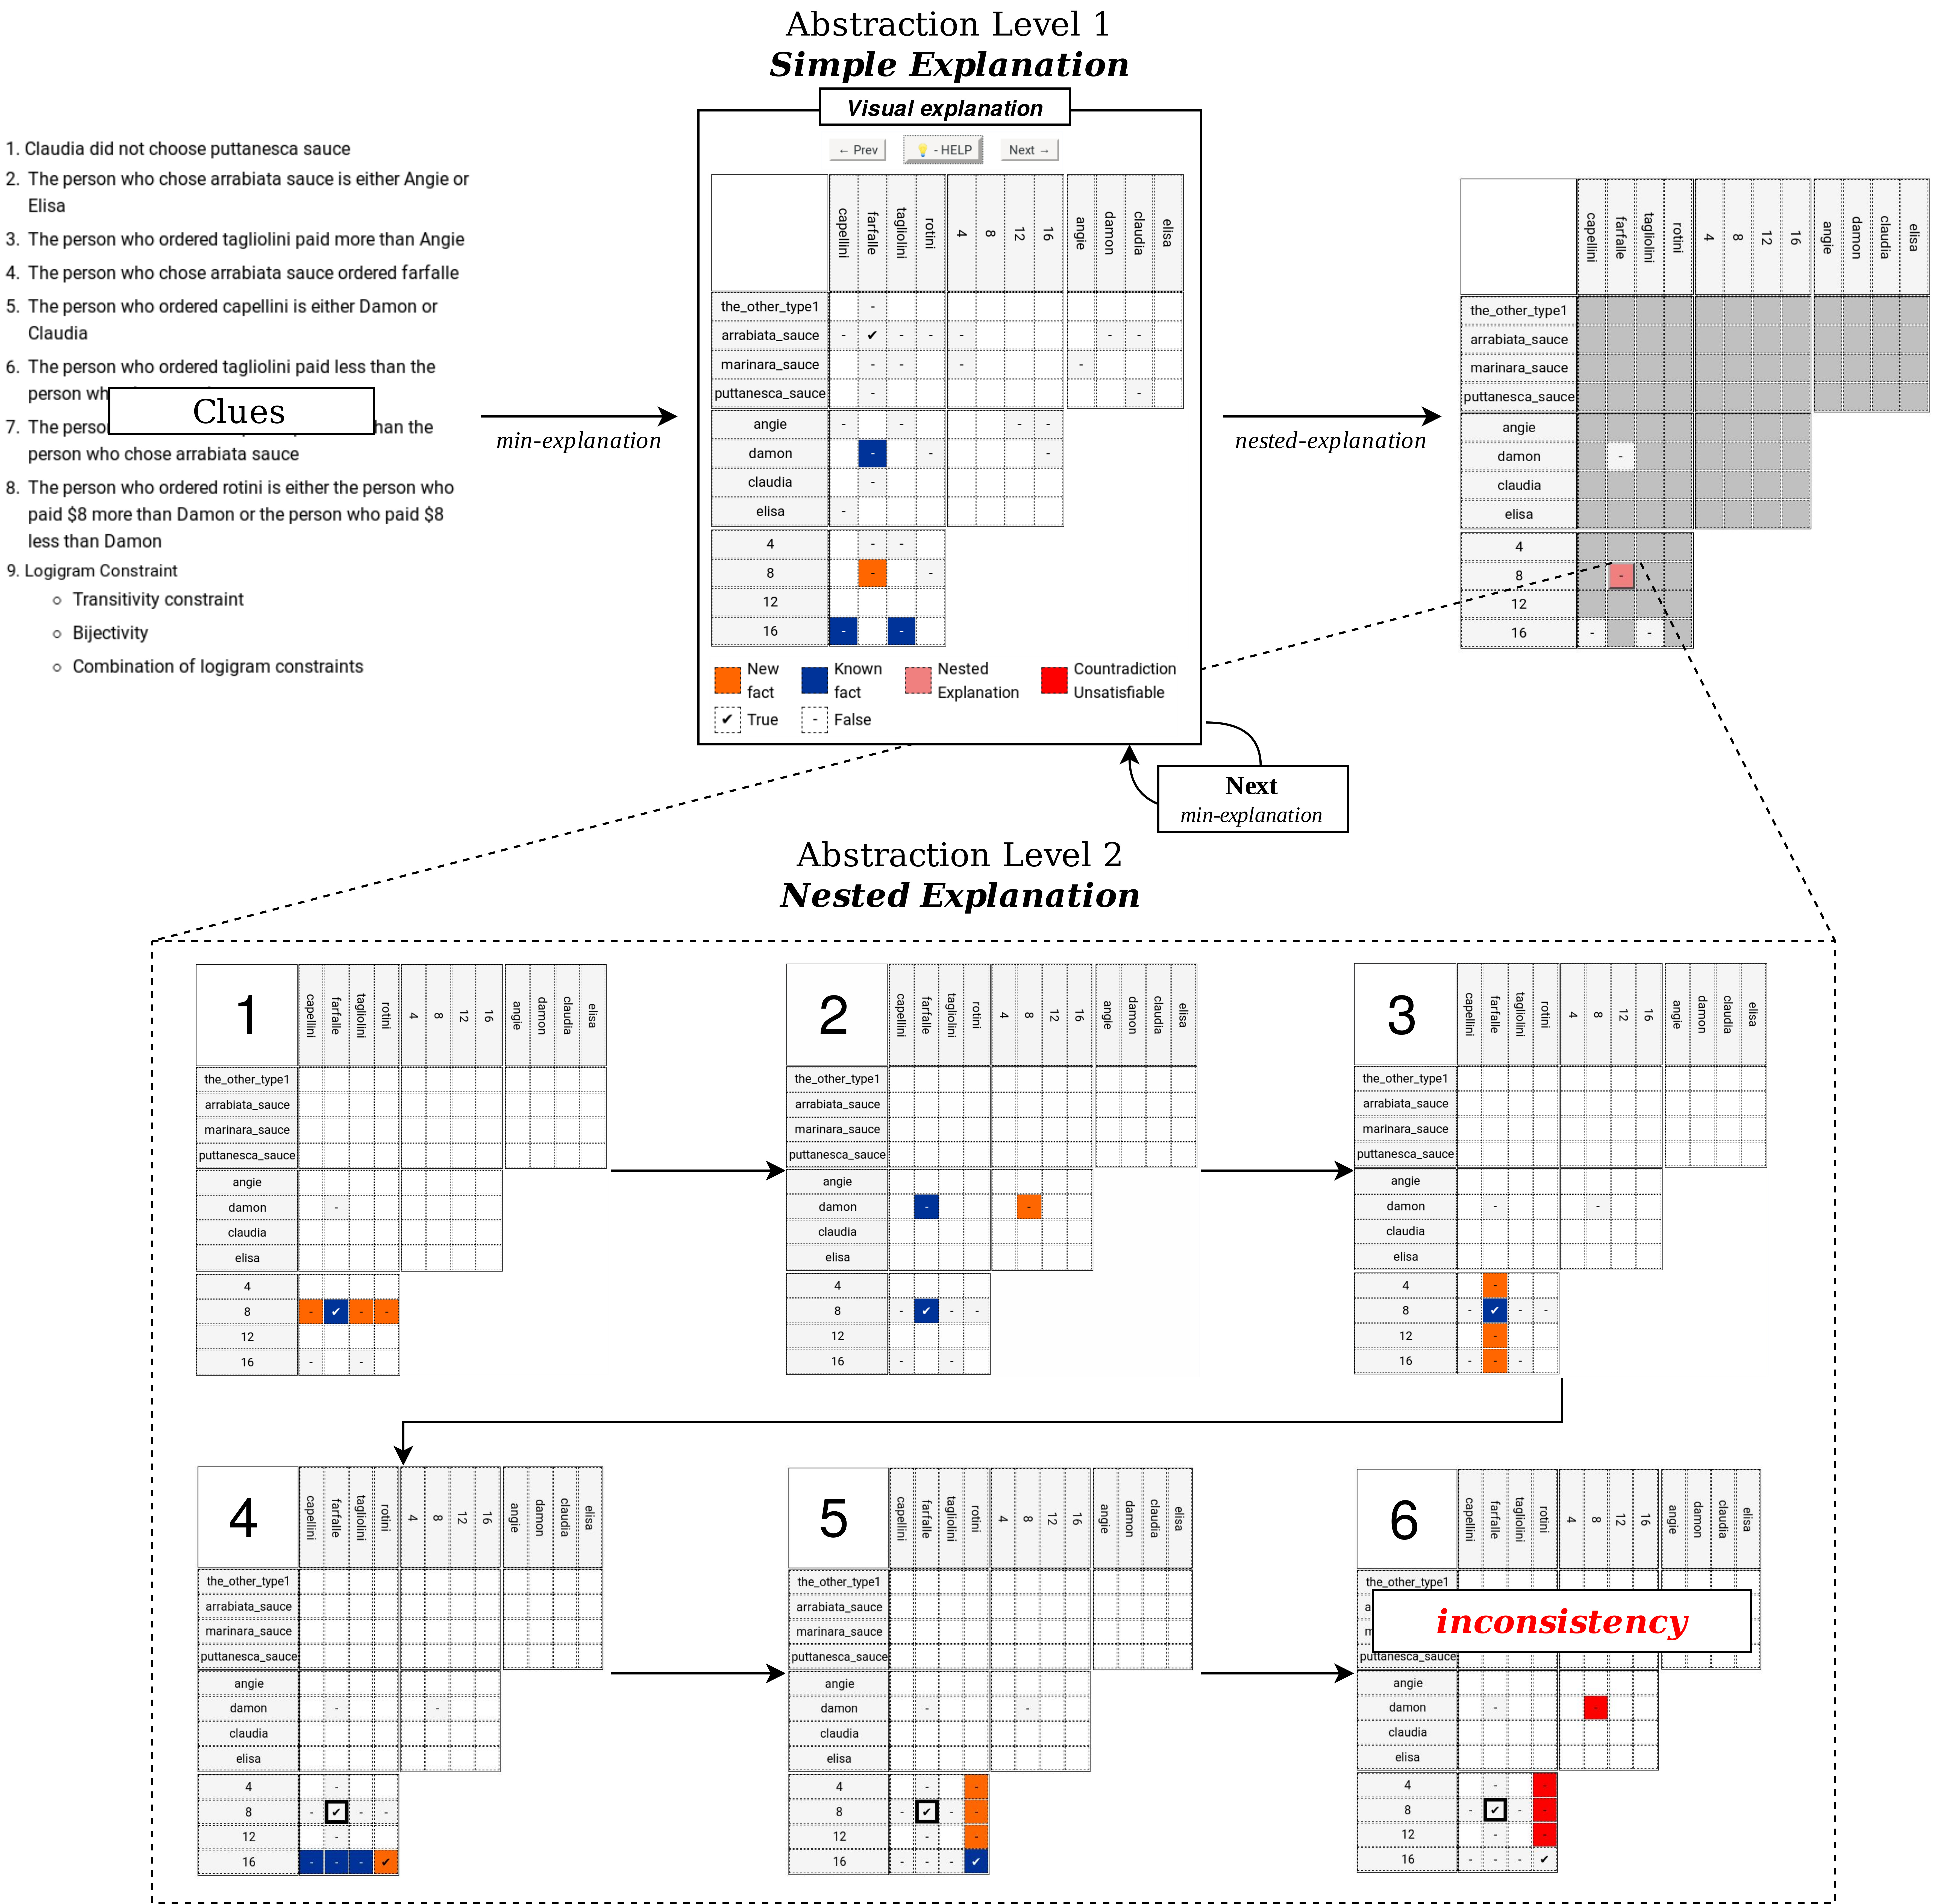
\includegraphics[width=\linewidth]{figures/inconsistency.jpg}
    \caption{\emilio{Small modification to the picture: Clues box higher, clue highlighted and reajusted box}A difficult explanation step, including its nested explanation}\label{fig:pasta_diff}
\end{figure}

We hence wish to provide a further, \textit{nested} explanation of such difficult reasoning steps. We believe that an explanation using contradiction is a good tool for this for two reasons: \emph{(i)} it is often used by people when solving puzzles, as well as by mathematicians when proving theorems; and \emph{(ii)} adding the negation of a derived fact such as `Farfalle does not cost \$8', allows us to generate a new sequence of non-redundant explanations up to inconsistency and hence contradiction, hence reusing the techniques from the previous section. 
This novel approach allows us to provide a mechanism for \emph{zooming in} into the most difficult explanation step.


%In this section, we extend the explanation-production problem with the purpose of refining those explanations that are too complex and taking inspiration from counterfactual reasoning.
% As such, our problem becomes an explanation-generating problem with 2 levels of abstractions: ``regular'' explanations and ``lower-level'' \textit{nested explanations}. \tias{lower-level is always 'by contradiction'? Maybe we should be more explicit about that?}

\myparagraph{Nested explanation of a reasoning step}


% To tackle complex inference steps with the lense of counterfactual reasoning, one  \textit{``Can I find another easier way to explain this step using the same facts and constraints by negating the newly derived fact and finding an inconsistency ?''} 


% For the definition of \textit{inconsistency}, we refer back to definition \ref{def:consistent}.


% Tias commented some (filler?) sentences
%The generation of the explanation sequence, as formally defined in Section 4, is initially guided by the cost function $f(E, S, N)$, a proxy for the mental-effort of the explanation-step. 
%To further explain the complex inference steps generated in the explanation sequence, w
%\tias{The nested explanation is by definition by contradiction due to the construction of I'0 and that I'n is inconsistent; I think we should be more explicit about this! It is not just nested (e.g. an abstraction level, with smaller steps)?}

%When should an explanation-step have a more detailed nested explanation of a newly derived fact?
We propose the following principles for what constitutes a meaningful and simple nested explanation, given a non-trivial explanation $(E,S,N)$:
%Each explanation $(E,S,N)$ might 
%For each explanation, we 
%Put differently, for every newly derived fact of a given explanation step $(E, S, N)$, we look for an \emph{nested} explanation sequence such that 
\begin{itemize}
 \item a nested explanation starts from the explaining facts $E$, %used in the parent explanation step, 
 augmented with the counterfactual assumption of a newly derived fact $n \in N$; 
 \item at each step, it only uses clues from $S$;
 \item each step is easier to understand (has a strictly lower cost) than the parent explanation which has cost $f(E,S,N)$;
 \item from the counterfactual assumption, a contradiction is derived. %; and
 %\item as before, a means to aggregate costs of the different steps to obtain a cost of the sequence to be minimized is assumed to exist.
\end{itemize}

Note that if an explanation steps derives multiple new facts, e.g. $|N| > 1$, then we can compute a nested explanation for each $n_i \in N$.

More formally, we define the concept of \emph{nested explanation} as follows:

\begin{definition}\label{def:nested-problem}
The \textbf{nested explanation} problem consists of --- given a non-redundant explanation $(E, S, N)$, and a newly derived fact $n \in N$ --- finding a non-redundant explanation sequence 
    \[\langle \ (I_0',(\emptyset,\emptyset,\emptyset)),\ (I_1',(E_1',S_1',N_1')), \dots ,\ (I_n',(E_n',S_n',N_n')) \ \rangle\]
    such that:
    \begin{itemize}
        \item $I_0'$ is the partial interpretation $\{ \neg n_i \wedge E \}$;
        \item $S_i'\subseteq S$ for each $i$;
        \item $f(E_i',S_i',N_i')< f(E, S, N)$ for each $i$; 
        \item $I_n'$ is inconsistent; and
        \item a predefined aggregate over the sequence $\left(f(E_i',S_i',N_i')\right)_{i\leq n}$ is minimised.
    \end{itemize}
\end{definition}

We can hence augment each explanation $(E,S,N)$ with a set of nested explanations if they exist. We next discuss algorithms for computing explanations and nested explanations.
%As for a regular explanation sequence, possible aggregation operators are \textit{max()} and \textit{average()}. 
%\noindent In the following section, we discuss algorithms to generate (nested) explanation sequences; afterwards, we apply them to the domain of logic grid puzzles.


% Ideas : 
% \begin{itemize}
%     \item During analysis of sequence of reasoning steps too hard/ complex to understand 
%     \item 2 levels of abstraction
%     \item Refine explanations using counterfactual reasoning
%     \item 
% \end{itemize}

% We introduce a second
